\documentclass{article}
\usepackage[utf8]{inputenc}
\usepackage{amsmath}
\usepackage{amssymb}
%\usepackage{pythontex}
\usepackage{minted}
\usepackage{xcolor} % to access the named colour LightGray
\usepackage{geometry}
\usepackage{graphicx}
\usepackage{tcolorbox}


\title{Python Project File}
\author{Soumya Majhi}
\date{January 2022}

\geometry{a4paper,
 %total={170mm,257mm},
 left=30mm,
 right=30mm,
 top=30mm,
 bottom=30mm
 }

\begin{document}

\maketitle
\begin{center}
    
\includegraphics[width=10cm, height=10cm]{images/python_logo.png}
\end{center}


\begin{tcolorbox}[colback=blue!5!white,colframe=blue!75!black]
    \begin{center}
        %\textbf{\huge{University Of Calcutta}} \\
        %\bigskip
        \Large{CC5 Practical Lab Notebook} \\
        \bigskip
        \large{Stream: B.Sc \\
        \bigskip
        Shift: Day \\
        \bigskip
        Department: Physics \\
        \bigskip
        Subject Code: PHSA \\
        \bigskip
        College Roll: 2817 \\
        \bigskip
        University Roll No.: 203224-21-0011 \\
        \bigskip
        University Registration No.: 224-1111-0520-20
        }
    \end{center}
\end{tcolorbox}

\newpage

{\Large\tableofcontents}

\footnote{This project is made with LaTeX}

\newpage

\section{Roots Of A Given Equation}
\subsection{Analytical Method}
Here, we just use the theory to find the root by graph plotting calculation.
\definecolor{LightGray}{gray}{0.9}
\begin{minted}
[frame=lines,baselinestretch=1.2, bgcolor=LightGray]
{python}
def f(x): return x**2-96.0  #defining a function
x=0.0
t=0.0001
while f(x)<0.0001:  #it will run until it crosses 0.0001
    x=x+t
print(x, f(x))
\end{minted}

\definecolor{LightGray}{gray}{0.9}
\begin{minted}
[frame=lines,baselinestretch=1.2, bgcolor=LightGray]
{python}
OUTPUT
9.797999999990504 0.0008039998139111049
\end{minted}

\subsection{Bisection Method}
If a function $f(x)$ is continuous between $x=a$ and b, and $f(a)$ and $f(b)$ are of opposite signs, then there exists a root between the a and b. Let us think that the root is at $x = \xi$ so that $f(\xi) = 0$

The root is found between a and b when $\boxed{f(a)f(b) < 0}$. The root can be approximated by the mid point, 
\begin{equation}
    \boxed{x_m = \frac{a+b}{2}} 
\end{equation}
That means we bisect the interval. Now in case, $f(x_m) = 0$, then that is the root. If not, we search the root in either of the interval $[a, x_m]$ or $[x_m, b]$.

In case, $f(a)f(b)<0$, the root lies in this half, otherwise in another. Then, as before, we bisect the new interval and repeat the process until the root is found according to accuracy.
\definecolor{LightGray}{gray}{0.9}
\begin{minted}
[frame=lines,baselinestretch=1.2, bgcolor=LightGray]
{python}
import sys
def f(x): return x**2-4.0
a=float(input("enter lower limit: "))
b=float(input("enter upper limit: "))
if f(a)*f(b)>0:
    print("No root is available within this range")
    sys.exit()
while abs(a-b)>=0.001:
    xm=(a+b)*0.5
    if f(xm)==0:
        print("Root = ",xm)
        sys.exit()
    if f(a)*f(xm)<0:
        b=xm                              #Left Half
    else:
        a=xm                              #Right Half
print("Root = ", (a+b)*0.5)
\end{minted}

\definecolor{LightGray}{gray}{0.9}
\begin{minted}
[frame=lines,baselinestretch=1.2, bgcolor=LightGray]
{python}
OUTPUT-1
enter lower limit: 5
enter upper limit: 6
No root is available within this range
\end{minted}

\definecolor{LightGray}{gray}{0.9}
\begin{minted}
[frame=lines,baselinestretch=1.2, bgcolor=LightGray]
{python}
OUTPUT-2
enter lower limit: 1
enter upper limit: 5
Root =  2.0
\end{minted}

\subsection{Newton-Raphson Method}
\textbf{Theory:} This method is an improved version of Bisection method. If $x_0$ is the approximate root of the equation: $f(x) = 0$, we can expand the function in Taylor's series around that point. Suppose, $x_1 = x_0 + h$ be the correct root, so that $f(x_1) = 0$. Taylor's series expansion: \\
\begin{equation}
    f(x_0 +h) = 0 = f(x_0) + hf'(x_0) + \frac{h^2}{2!}f''(x_0) +...
\end{equation}
Neglecting the terms with second and higher order derivatives, we have,
\begin{equation}
    f(x_0) + hf'(x_0) = 0 \\
    \Rightarrow h = -\frac{f(x_0)}{f'(x_0)}
\end{equation}
Thus, an approximation of the root can be $x_1 = x_0 -\frac{f(x_0)}{f'(x_0)}$. \\
Given an initial approximation $x_0$, we can generate $x_1$ and then successively, $x_2, x_3,...$ in order to reach closer and closer to the root. \\
Therefore, we get the \textbf{Newton-Raphson formula} as:
\begin{gather}
    \boxed{x_{n+1} = x_n - \frac{f(x_n)}{f'(x_n)}}
\end{gather}
\definecolor{LightGray}{gray}{0.9}
\begin{minted}
[frame=lines,baselinestretch=1.2, bgcolor=LightGray]
{python}
import sys
def f(x):return x**2-4.0                             #function
def h(x):return 2*x                                  #derivative
x=float(input("enter the value of approximate root: "))
if f(x)==0:
	print("Root = ", x)
	sys.exit()
while f(x)>0.0001:
	x=x-f(x)/h(x)
print("Root = ", x)
\end{minted}

\definecolor{LightGray}{gray}{0.9}
\begin{minted}
[frame=lines,baselinestretch=1.2, bgcolor=LightGray]
{python}
OUTPUT
enter the value of approximate root: 5
Root =  2.0000051812194735
\end{minted}

\section{Interpolation}
\subsection{Newton's Forward Interpolation}
Newton's Interpolation (also called \emph{Gregory-Newton} Interpolation) is done through a simple polynomial of degree $n$ for a set of $(n +1)$ equidistant data points: $(x_0,y_0), (x_1,y_1),..., (x_n,y_n)$. Consider, $x_i = x_0 +ih, i=0,1,2,...n.$
So, \textbf{Newton's Interpolation Formula} with \textbf{forward differences} is: \\

\fbox{
 \addtolength{\linewidth}{-2\fboxsep}%
 \addtolength{\linewidth}{-2\fboxrule}%
 \begin{minipage}{\linewidth}
    \begin{multline}
        \Phi(x) = y_0 + t{\Delta}y_0 + \frac{t(t-1)}{2!}{\Delta}^2y_0 + \frac{t(t-1)(t-2)}{3!}{\Delta}^3y_0 +...\\
        + \frac{t(t-1)(t-2)...(t-n+1)}{n!}{\Delta}^ny_0
    \end{multline}
 \end{minipage}
}
where, $t = \frac{x-x_0}{h}$
\definecolor{LightGray}{gray}{0.9}
\begin{minted}
[frame=lines,baselinestretch=1.2, bgcolor=LightGray]
{python}
x=[5.0,10.0,15.0,20.0,25.0,30.0]
y=[45.0,105.0,174.0,259.0,364.0,496.0]
d=[]
xn = float(input("enter a value of x: "))
t=(xn-x[0])/5.0 
sum=y[0]
coef=t
k=1.0
for i in range(len(y),1,-1):
	for j in range(i-1):
		dif=y[j+1]-y[j]
		d.append(dif)
	sum=sum+coef*d[0]
	coef=(coef*(t-k))/(k+1)     #updating the coef
	k=k+1
	y=d
	d=[]
print("Interpolated Value = ", sum)
\end{minted}

\definecolor{LightGray}{gray}{0.9}
\begin{minted}
[frame=lines,baselinestretch=1.2, bgcolor=LightGray]
{python}
OUTPUT
enter a value of x: 18
Interpolated Value =  222.826688
\end{minted}

\subsection{Newton's Backward Interpolation}
\textbf{Newton's Interpolation} formula with \textbf{backward differences} is:
\begin{align}
    \boxed{\Phi(x) = y_n + t{\nabla}y_n + \frac{t(t+1)}{2!}{\nabla}^2y_n + ...+ \frac{t(t+1)(t+2)...[t+(n-1)]}{n!}{\nabla}^ny_n}
\end{align}
\definecolor{LightGray}{gray}{0.9}
\begin{minted}
[frame=lines,baselinestretch=1.2, bgcolor=LightGray]
{python}
x=[5.0,10.0,15.0,20.0,25.0,30.0]
y=[45.0,105.0,174.0,259.0,364.0,496.0]
d=[]
xn = float(input("enter a value of x: "))
n=len(x)-1
t=(xn-x[n])/5.0
sum=y[n]
coef=t
k=1.0
for i in range (len(y),1,-1):
	for j in range(i-1):
		dif=y[j+1]-y[j]
		d.append(dif)
	sum=sum+coef*d[j]
	coef=(coef*(t+k))/(k+1)
	k=k+1
	y=d
	d=[]
print("Interpolated Value = ", sum)
\end{minted}

\definecolor{LightGray}{gray}{0.9}
\begin{minted}
[frame=lines,baselinestretch=1.2, bgcolor=LightGray]
{python}
OUTPUT
enter a value of x: 18
Interpolated Value =  222.826688
\end{minted}

\section{Integration}
\subsection{Rectangular Method}
This is the simplest case. Here we have, $h=b-a$ and $f(x)\approx\Phi(x) = y_0$.
\begin{equation}
    \therefore \boxed{I \approx \int_a^b \Phi(x)dx = hy_0}
\end{equation}
Applying \textbf{rectangle rule} for integration over each sub-interval, $h=(b-a)/n$, we get a \textbf{Composite formula}:
\begin{equation}
    \boxed{I = \int_{x_0}^{x_n} ydx = h[y_0+y_1+y_2+...+y_{n-1}]}
\end{equation}
\definecolor{LightGray}{gray}{0.9}
\begin{minted}
[frame=lines,baselinestretch=1.2, bgcolor=LightGray]
{python}
def f(x): return 3.0
b=float(input('enter upper limit'))
a=float(input('enter lower limit'))
sum=f(a)*(b-a)
print("Value of Integral = ", sum)
\end{minted}

\definecolor{LightGray}{gray}{0.9}
\begin{minted}
[frame=lines,baselinestretch=1.2, bgcolor=LightGray]
{python}
OUTPUT
enter upper limit6
enter lower limit2
Value of Integral = 12.0
\end{minted}

\subsection{Trapezoidal Rule}
\textbf{Formula:} 
\begin{equation*}
    \int_a^b \Phi(x) dx = \frac{h}{2}(y_0 + y_1)
\end{equation*}
\textbf{Theory:} Here $n = 1, x_0 = a, x_1 = b$ and $f(x) \approx \Phi(x) = y_0 + t\Delta{y_0}$ \\
\begin{gather}
    \therefore I = \int_a^b \Phi(x)dx = \int_a^b [y_0 + t\Delta{y_0}]dx \\
    = \int_a^b[y_0 + t(y_1 - y_0)]hdt \\
    =hy_0 + h(y_1-y_0).\frac{1}{2} \\
    \boxed{I =\frac{h}{2}(y_0 + y_1)} 
\end{gather}
The value of the integral is the area of the \textit{trapezium} with base h=b-a and bounded by the ordinates $y_0$ and $y_1$.
\definecolor{LightGray}{gray}{0.9}
\begin{minted}
[frame=lines,baselinestretch=1.2, bgcolor=LightGray]
{python}
def f(x): return x
b=float(input('enter upper limit: '))
a=float(input('enter lower limit: '))
h=b-a
sum= 0.5*(f(a)+f(b))*h
print("Value of Integral = ",sum)
\end{minted}

\definecolor{LightGray}{gray}{0.9}
\begin{minted}
[frame=lines,baselinestretch=1.2, bgcolor=LightGray]
{python}
OUTPUT
enter upper limit: 6
enter lower limit: 2
Value of Integral = 16.0
\end{minted}

\subsubsection{Composite Trapezoidal Rule}
\textbf{Formula:}
\begin{equation*}
    \int_{x_0}^{x_n} f(x)dx = \frac{h}{2}[y_0 + 2(y_1+y_2+...+y_{n-1}) + y_n] 
\end{equation*}
\textbf{Theory:} We can apply the trapezoidal rule over each of the sub-intervals and achieve the composite formula. \\
\begin{gather}
    I = \int_{a=x_0}^{b=x_n}f(x)dx = \int_{x_0}^{x_1}f(x)dx + \int_{x_1}^{x_2}f(x)dx +...+ \int_{x_{n-1}}^{x_n}f(x)dx \\
    = \frac{h}{2}(y_0 + y_1) + \frac{h}{2}(y_1 + y_2)+...+\frac{h}{2}(y_{n-1}+y_n) \\
    \boxed{I = \frac{h}{2}[(y_0 + y_n) + 2(y_1 + y_2 + y_3 +...+y_{n-1})]}
\end{gather}
\definecolor{LightGray}{gray}{0.9}
\begin{minted}
[frame=lines,baselinestretch=1.2, bgcolor=LightGray]
{python}
def f(x): return x**2
b=float(input('enter upper limit: '))
a=float(input('enter lower limit: '))
n=int(input('enter no of division: '))
h=(b-a)/n
sum=(f(b)+f(a))*0.5
for i in range (1,n):
	x=a+i*h
	sum=sum+f(x)
print("Value of Integral = ", h*sum)
\end{minted}

\definecolor{LightGray}{gray}{0.9}
\begin{minted}
[frame=lines,baselinestretch=1.2, bgcolor=LightGray]
{python}
OUTPUT
enter upper limit: 10
enter lower limit: 2
enter no of division: 100
Value of Integral =  330.67519999999996
\end{minted}

\subsection{Simpson's $\frac{1}{3}$ Rule}
\textbf{Formula:} 
\begin{equation*}
    \int_{a}^{b}\Phi(x) dx = \frac{h}{3}[y_0 +4y_1 + y_2]
\end{equation*}
\textbf{Theory:} For two sub-intervals, i.e., $n=2$, we consider upto ${\Delta}^2y_2$ term. So, we must consider three points, say, $(x_0,y_0), (x_1,y_1), (x_2,y_2)$. \\
If we consider $x_0 = a$ and $x_2 = b$, then $x_1 = \frac{a+b}{2}$ (the mid-point), then, \\
\begin{gather}
    \therefore I \approx \int_a^b \Phi(x) dx = \int_a^b [y_0 + t{\Delta}y_0 + \frac{t(t-1)}{2!}{\Delta}^2y_0]dx \\
    = \int_0^2[y_0 + t(y_1 - y_0)+\frac{(t^2 - t)}{2}(y_2 - 2y_1 + y_0)]hdt \\
    \boxed{I = \frac{h}{3}[y_0 +4y_1 + y_2]}
\end{gather}



\definecolor{LightGray}{gray}{0.9}
\begin{minted}
[frame=lines,baselinestretch=1.2, bgcolor=LightGray]
{python}
def f(x): return x**2
b=float(input('enter upper limit: '))
a=float(input('enter lower limit: '))
h=(b-a)/2
y0=f(a)
y1=f(0.5*(a+b))
y2=f(b)
sum= (h/3.0)*(y0+4*y1+y2)
print("Value of Integral =  ", sum)
\end{minted}

\definecolor{LightGray}{gray}{0.9}
\begin{minted}
[frame=lines,baselinestretch=1.2, bgcolor=LightGray]
{python}
#OUTPUT
enter upper limit: 10
enter lower limit: 2
Value of Integral = 330.66666666666663
\end{minted}

\subsubsection{Composite Simpson's $\frac{1}{3}$ Rule}
\textbf{Formula:} 
\begin{equation*}
    \int_{x_0}^{x_n} ydx = \frac{h}{3}[y_0 +4(y_1+y_3+...+y_{n-1}) +2(y_2 +y_4 +... +y_{n-2}) +y_n]
\end{equation*}
\textbf{Theory:} For Simpson's $\frac{1}{3}$ rule to be applied between two points, we require two equally spaced sub-intervals, each of length $h$. So, the rule requires the division of the whole range $[a,b]$ into an even number of sub-intervals of width $h$. \\
To be explicit, we have two sub-intervals given by the three given consecutive points $(x_0,y_0), (x_1, y_1), (x_2, y_2)$, over which we apply Simpson's $\frac{1}{3}$ rule. \\
So, \\
\begin{equation*}
    \int_{x_o}^{x_2} ydx = \frac{h}{3} [y_0 + 4y_1 + y_2]
\end{equation*}
   
Similarly, for the next sub-intervals $\rightarrow$ 
\begin{gather}
    \therefore I = \int_{x_0}^{x_n} ydx = \frac{h}{3}[(y_0 + 4y_1 + y_2) + (y_2 +4y_3 +y_4) + ... + (y_{n-2} +4y_{n-1} + y_n)] \\
    \boxed{I = \frac{h}{3}[y_0 +4(y_1+y_3+...+y_{n-1}) +2(y_2 +y_4 +... +y_{n-2}) +y_n]}
\end{gather}

\definecolor{LightGray}{gray}{0.9}
\begin{minted}
[frame=lines,baselinestretch=1.2, bgcolor=LightGray]
{python}
def f(x): return x**2
b=float(input('enter upper limit: '))
a=float(input('enter lower limit: '))
n=int(input('enter number of division: '))
h=(b-a)/n
sum1=f(a)+f(b)
sum2=0.0
for i in range (1,n,2):
	x=a+i*h
	sum2=sum2+f(x)
sum3=0.0
for j in range (2,n,2):
	x=a+j*h
	sum3=sum3+f(x)
I=(h/3.0)*(sum1+(4*sum2)+(2*sum3))
print("Value of Integral = ", I)
\end{minted}

\definecolor{LightGray}{gray}{0.9}
\begin{minted}
[frame=lines,baselinestretch=1.2, bgcolor=LightGray]
{python}
OUTPUT
enter upper limit: 10
enter lower limit: 2
enter number of division: 10
Value of Integral =  330.6666666666667
\end{minted}

\subsection{Integration by SciPy Module}
The module \texttt{integrate} in \texttt{SciPy} consists of various functions to do integration. For example, \texttt{trapz} for Trapezoidal rule and \texttt{simps} for Simpson's rule.
\definecolor{LightGray}{gray}{0.9}
\begin{minted}
[frame=lines,baselinestretch=1.2, bgcolor=LightGray]
{python}
import numpy as np
from scipy import integrate
x=np.arange(2,11)
y = x**2
I=integrate.simps(y,x)
print("Value of Integral =  ", I)
\end{minted}

\definecolor{LightGray}{gray}{0.9}
\begin{minted}
[frame=lines,baselinestretch=1.2, bgcolor=LightGray]
{python}
OUTPUT
Value of Integral =   330.66666666666663
\end{minted}

\section{Ordinary Differential Equations}
\subsection{Euler's Method}
\textbf{Theory:} Let us consider a general first order differential equation,
$\frac{dy}{dx} = f(x,y)$ with an initial condition $y(x_0) = y_0$. \\
We want to solve the differential equation for y at different values of x. Consider, these points are $x_n = x_0 + nh$ , $n = 1,2,3,...$ Between the first two points $[x_0, x_1]$, \\
\begin{equation}
    y_1 = y_0 + \int_{x_0}^{x_1} f(x,y)dx
\end{equation}
If we assume, $f(x,y) = f(x_0, y_0)$, we get an approximate formula: 
\begin{equation}
    y_1 = y_0 + hf(x_0,y_0)
\end{equation}
where, $h=x_1 -x_0$. Note that the integration is done by \textit{Rectangle rule}. \\
Similarly, for the next range $[x_1, x_2]:$ \\
\begin{gather}
    y_2 = y_1 + hf(x_1, y_1)
\end{gather}
So, General \textbf{Euler's formula} is $\rightarrow$
\begin{gather}
   \boxed{y_{n+1} = y_n + hf(x_n, y_n)}
\end{gather}
\definecolor{LightGray}{gray}{0.9}
\begin{minted}
[frame=lines,baselinestretch=1.2, bgcolor=LightGray]
{python}
def f(x,y):return 3*x*y         #Defining the function
x, y = 0.0, 1.0                 #Initial values
h=0.01                          #Step size
for i in range(201):
	y=y+h*f(x,y)            #Updating by Euler's formula
	x=x+h
print(x, y)
\end{minted}

\definecolor{LightGray}{gray}{0.9}
\begin{minted}
[frame=lines,baselinestretch=1.2, bgcolor=LightGray]
{python}
OUTPUT
2.010000000000001 369.6691477543691
\end{minted}


\subsection{Runge-Kutta 2$^{nd}$ Order (RK2)}
\textbf{Theory:} We consider the integral,
\begin{equation}
    y_1 = y_0 + \int_{x_0}^{x1}f(x,y)dx
\end{equation}
In Euler's method, we approximated this by Rectangle rule obtaining the expression: $y_1 \approx y_0 +hf(x_0, y_0)$.\\
Now, we can do a better approximation of the integral by Trapezoidal rule:
\begin{gather}
    y_1 = y_0 + \frac{h}{2}[f(x_0,y_0)+f(x_1,y_1)] \\
    y_1 = y_0 + \frac{h}{2}[f(x_0,y_0)+f(x_0+h,y_0+hf_0)] \\
    y_1 = y_0 + \frac{h}{2}[f_0+f(x_0+h,y_0+hf_0)] \\
    \boxed{= y_0 + \frac{1}{2}[k_1+k_2]}
\end{gather}
Here, 
\begin{gather*}
    \boxed{k_1=hf_0, k_2=hf(x_0+h, y_0 +hf_0)}
\end{gather*}

\definecolor{LightGray}{gray}{0.9}
\begin{minted}
[frame=lines,baselinestretch=1.2, bgcolor=LightGray]
{python}
def f(x,y):return 3*x*y
x,y = 0.0, 1.0
h = 0.01
for i in range(201):
	k1=h*f(x,y)
	k2=h*f(x+h,y+k1)
	y=y+0.5*(k1+k2)
	x=x+h
print(x,y)
\end{minted}

\definecolor{LightGray}{gray}{0.9}
\begin{minted}
[frame=lines,baselinestretch=1.2, bgcolor=LightGray]
{python}
OUTPUT
2.010000000000001 427.68060123959447
\end{minted}

\subsection{Runge-Kutta 4$^{th}$ Order (RK4)}
\textbf{Theory:} Commonly used formulas of \textbf{$4^{th}$ order} Runge-Kutta (RK4) method are:

\begin{equation}
    \boxed{
        \begin{gathered}
            k_1 = hf(x_0,y_0) \\
            k_2 = hf(x_0 + \frac{h}{2}, y_0 + \frac{k_1}{2}) \\
            k_3 = hf(x_0 + \frac{h}{2}, y_0 + \frac{k_2}{2}) \\
            k_4 = hf(x_0 + h, y_0 + k_3) \\
            y_1 = y_0 + \frac{1}{6}(k_1 + 2k_2 + 2k_3 + k_4)
        \end{gathered}
    }
\end{equation}

\definecolor{LightGray}{gray}{0.9}
\begin{minted}
[frame=lines,baselinestretch=1.2, bgcolor=LightGray]
{python}
def f(x,y): return 3*x*y
x,y = 0.0, 1.0
h = 0.01
for i in range(201):
	k1=h*f(x,y)
	k2=h*f(x+h*0.5,y+k1*0.5)
	k3=h*f(x+h*0.5,y+k2*0.5)
	k4=h*f(x+h,y+k3)
	y=y+(k1+2*k2+2*k3+k4)/6.0
	x=x+h
print(x, y)
\end{minted}

\definecolor{LightGray}{gray}{0.9}
\begin{minted}
[frame=lines,baselinestretch=1.2, bgcolor=LightGray]
{python}
OUTPUT
2.010000000000001 428.4396065649443
\end{minted}

\appendix
\section{Comparison of Euler's, RK2 \& RK4 Methods}
\definecolor{LightGray}{gray}{0.9}
Let us now write a python program for all methods of solving ODE, together. We plot graphically to compare the various methods.
\begin{minted}
[frame=lines,baselinestretch=1.2, bgcolor=LightGray]
{python}
import matplotlib.pyplot as plt
import numpy as np
import math
d=np.linspace(0,2.01,201)
d3=np.exp(1.5*d**2)
d1=[]
d2=[]
d4=[]
#Euler Method
def f(x,y): return 3*x2*y2
x2=0.0
y2=1.0
h=0.01
for i in range (201):
	y2=y2+h*f(x2,y2)
	x2=x2+h
	d4.append(y2)
print (y2)
#Rk 2 Method 
def f(x,y): return 3*x*y
x=0.0
y=1.0
h=0.01
for i in range (201):
	k1=h*f(x,y)
	k2=h*f(x+h,y+k1)
	y=y+0.5*(k1+k2)
	x=x+h
	d1.append(y)
print (y)
#RK-4 Method
def f(x,y): return 3*x1*y1
x1=0.0
y1=1.0
h=0.01
for i in range (201):
	k11=h*f(x1,y1)
	k22=h*f(x1+h/2.0,y1+k11/2.0)
	k3=h*f(x1+h/2.0,y1+k22/2.0)
	k4=h*f(x1+h,y1+k3)
	y1=y1+(1/6.0)*(k11+2*k22+2*k3+k4)
	x1=x1+h
	d2.append(y1)
print (y1)
plt.plot(d,d1,'*',label='RK2')
plt.plot(d,d2,'.',label='RK4')
plt.plot(d,d3,label='EXACT') 
plt.plot(d,d4,'+',label='EULER')
plt. legend(fontsize=10) 
plt.show()
\end{minted}


\begin{figure}[ht]
    %\centering
    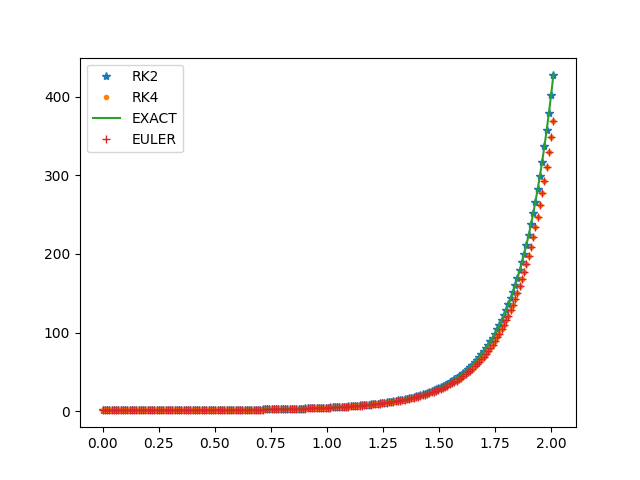
\includegraphics{images/Figure_1.png}
    \caption{Graphical plot of Euler's, RK2 \& Rk4 Methods}
\end{figure}



\end{document}